%% =====================================================================
%%  FIT-ARCADE — Sensing & Adaptive-Personalization journal manuscript
%%  Target venue: IEEE Journal of Biomedical and Health Informatics (JBHI)
%%  Class: IEEEtran (journal, two-column, 10pt)
%%  Build:  pdflatex main && bibtex main && pdflatex main && pdflatex main
%%
%%  SCOPE: sensing (motion-gated rPPG), effort fusion, personalized closed-loop
%%  difficulty, and empirical evaluation ONLY. The platform ARCHITECTURE is a
%%  black box cited to the companion SDPS paper [fitarcade-sdps]; never re-described.
%% =====================================================================
\documentclass[journal,10pt]{IEEEtran}

\usepackage{amsmath,amssymb,amsfonts}
\usepackage{algorithm}
\usepackage[noend]{algpseudocode}
\usepackage{graphicx}
\usepackage{booktabs}
\usepackage{array}
\usepackage{xcolor}
\usepackage{tikz}
\usetikzlibrary{arrows.meta,positioning,fit,calc,backgrounds}
\usepackage{url}
\usepackage[hidelinks]{hyperref}

% --- Draft markers: RED = author task, BLUE = value to fill once data exist ---
\newcommand{\todoNote}[1]{\textcolor{red}{\textbf{[TODO:} #1\textbf{]}}}
\newcommand{\result}[1]{\textcolor{blue}{\underline{#1}}}
\newcommand{\ph}[1]{\textcolor{blue}{$\langle$#1$\rangle$}}   % study parameter placeholder

% --- Convenience ---
\newcommand{\ssystem}{\textsc{FIT-ARCADE}}
\newcommand{\hmax}{\mathrm{HR}_{\max}}
\newcommand{\hrrest}{\mathrm{HR}_{\mathrm{rest}}}
\newcommand{\clip}{\operatorname{clip}}

\begin{document}

\title{Motion-Robust Contactless Heart-Rate Sensing and\\ Personalized Closed-Loop Difficulty for\\ Markerless Exergames}

\author{% \todoNote{author list --- reuse SDPS authors unless told otherwise}
        [AUTHOR\_LIST]% e.g. First Author, Second Author, \IEEEmembership{Member,~IEEE}
        \thanks{Manuscript submitted \todoNote{date}. \emph{(Corresponding author: [CORRESPONDING\_EMAIL].)}}%
        \thanks{The authors are with [AFFILIATION] (e-mail: [CORRESPONDING\_EMAIL]).}%
        \thanks{The decoupled software architecture of the exergaming platform used here is described in a companion paper~\cite{fitarcade-sdps}; this article concerns only its sensing and adaptation subsystems.}}

\markboth{IEEE Journal of Biomedical and Health Informatics,~Vol.~XX, No.~X, 2026}%
{Author \MakeLowercase{\textit{et al.}}: Motion-Robust Contactless Heart-Rate Sensing for Markerless Exergames}

\maketitle

% =====================================================================
\begin{abstract}
Exergames couple physical activity to play, but sustaining an effective, safe
training intensity requires knowing how hard the player is working---information
normally obtained from wearable heart-rate (HR) sensors that add cost and
friction. Remote photoplethysmography (rPPG) can recover HR from an ordinary
webcam, yet the vigorous whole-body motion intrinsic to exergaming is precisely
what corrupts the rPPG signal. We present a wearable-free sensing and adaptation
pipeline that turns this liability into an asset: because a markerless exergame
already computes a body pose each frame, we \emph{reuse the pose skeleton} both to
place a stable forehead region of interest and, as our central contribution, to
\emph{gate and hold} the HR estimate during motion. A pluggable, extractor-agnostic
pulse pipeline (green-channel by default) with a non-uniform-timestamp periodogram
yields HR and a spectral confidence; a pose-derived motion level attenuates that
confidence and
freezes the estimate when the body moves too fast. HR reserve is fused with
markerless rep cadence into a single effort signal that drives a personalized,
closed-loop difficulty controller whose per-player baseline is set from age,
resting HR, and self-reported fitness. We specify the complete method---grounded
in a deployed browser implementation---and a rigorous human-subjects evaluation
spanning HR accuracy across the Fitzpatrick skin-tone scale and lighting, a
motion-gating ablation, comparison against green/CHROM/ICA/POS and a deep-learning
baseline, effort validity against \%HRR and Borg RPE, closed-loop efficacy versus
fixed difficulty, and cross-profile personalization. Key quantitative results are
reported as placeholders pending data collection. \result{Headline result placeholder.}
\end{abstract}

\begin{IEEEkeywords}
Remote photoplethysmography, contactless heart rate, motion artifact, markerless
sensing, adaptive difficulty, exergaming, human-in-the-loop control, personalization.
\end{IEEEkeywords}

% =====================================================================
\section{Introduction}
\IEEEPARstart{P}{hysical} inactivity is a leading modifiable risk factor for
non-communicable disease and premature mortality~\cite{who2020}. \emph{Exergames}
---video games driven by bodily motion---raise activity by embedding exercise in
play and have shown moderate-to-vigorous intensity comparable to conventional
training~\cite{exergame-meta}. Their health value, however, depends on the player
exercising at an \emph{appropriate and safe intensity}: too low wastes the
session, too high risks over-exertion, and the ideal band shifts with age and
fitness. Quantifying intensity in real time normally means strapping on a
heart-rate (HR) monitor---an added device, cost, and point of friction that
undermines the low-barrier promise of a webcam exergame.

Remote photoplethysmography (rPPG) recovers the cardiac pulse from subtle
skin-colour changes in ordinary video~\cite{verkruysse2008,poh2010,dehaan2013,wang2017},
raising the prospect of a fully contactless, wearable-free training loop. The
obstacle is fundamental: rPPG is a weak signal easily overwhelmed by motion
artifact~\cite{rppg-survey}, and exergaming is defined by vigorous, whole-body
motion. Consequently, the substantial literature on physiologically adaptive
exergames almost universally relies on a \emph{worn} HR sensor to close the loop,
while camera-based HR work has largely been confined to rest or gentle activity.
The intersection---closing an exertion-regulation loop using camera-only
physiology under the motion regime of real exergaming---is under-studied.

\textbf{Insight.} A markerless exergame \emph{already} runs a real-time body-pose
estimator to drive gameplay. We exploit this for sensing at zero additional cost:
(i) the face landmarks place a stable forehead region of interest (ROI) without a
separate face tracker, and (ii)---the key idea---the \emph{velocity of the pose
skeleton} is a direct, cheap proxy for exactly the motion that corrupts rPPG, so
we use it to gate the estimate's confidence and to \emph{hold} the last trusted
reading through bursts of vigorous movement. The very motion that defeats naive
rPPG becomes an observable that tells the estimator when \emph{not} to trust
itself.

\textbf{Contributions.}
\begin{enumerate}
\item A \emph{motion-gated, pose-reuse rPPG} method tailored to the exercise
regime: a forehead ROI from pose face landmarks, an extractor-agnostic pulse
pipeline (green-channel by default; POS/CHROM as baselines) with a
non-uniform-timestamp periodogram and spectral confidence, and a pose-velocity
motion gate that attenuates confidence and holds the estimate under vigorous
motion (Section~\ref{sec:rppg}).
\item A markerless \emph{effort} estimator fusing rep cadence with HR reserve,
confidence-gated with a cadence-only fallback when rPPG is untrustworthy
(Section~\ref{sec:effort}).
\item A \emph{personalized, closed-loop adaptive-difficulty} controller whose
per-player baseline is derived from age, resting HR, and fitness, and whose gain
is deliberately conservative to match human movement dynamics
(Section~\ref{sec:control}).
\item A \emph{rigorous empirical evaluation} design---accuracy across skin tone
and lighting, a motion-gating ablation, rPPG-baseline comparison, effort validity,
closed-loop efficacy, and cross-profile personalization
(Sections~\ref{sec:design}--\ref{sec:results}).
\end{enumerate}

The platform's software architecture (the decoupled ``motion-seam'' that lets the
sensing and adaptation modules described here drive heterogeneous games) is the
subject of a companion paper~\cite{fitarcade-sdps} and is treated here strictly as
a black box. The remainder of the paper is organized as follows.
Section~\ref{sec:related} reviews rPPG and adaptive exergaming;
Section~\ref{sec:overview} places the subsystems; Sections~\ref{sec:rppg}--\ref{sec:control}
detail the method; Sections~\ref{sec:design}--\ref{sec:results} present the
evaluation design and result placeholders; Sections~\ref{sec:discussion}--\ref{sec:conclusion}
discuss and conclude.

% =====================================================================
\section{Related Work}\label{sec:related}

\subsection{Remote Photoplethysmography and Motion Artifact}
rPPG evolved from spatial averaging of the green channel~\cite{verkruysse2008}
and blind source separation~\cite{poh2010} to model-based chrominance methods:
CHROM~\cite{dehaan2013} and the Plane-Orthogonal-to-Skin (POS)
projection~\cite{wang2017}, which are markedly more robust to illumination and
skin tone. Learning-based estimators such as DeepPhys~\cite{chen2018} and
PhysNet~\cite{yu2019} improve accuracy but require training data, add
computational cost, and can generalize poorly across skin tone and
device---concerns amplified in a browser deployment. Recent
surveys~\cite{rppg-survey} identify \emph{motion robustness} as the dominant open
problem: subject motion introduces artifacts spectrally overlapping the pulse.
Most mitigations operate \emph{within} the signal (adaptive filtering, ROI
re-selection). We instead add an \emph{exogenous} motion observable---pose
velocity---that the exergame already computes, and use it to gate rather than to
filter. \todoNote{cite 3--4 recent (2023--2025) JBHI rPPG / contactless-vitals
papers to anchor the target venue.}

\subsection{Effort Estimation and Adaptive Exergaming}
Closed-loop or ``biocybernetic'' games feed physiological state back into game
parameters~\cite{parnandi2013}. In exergaming, HR-zone dynamic difficulty
adjustment (DDA) regulates exertion and can improve time-in-zone, perceived
exertion, and enjoyment relative to non-adaptive
play~\cite{hrdda-vrst,cardio-personalization}. Effort/intensity has also been
estimated by fusing HR with accelerometry or vision-based energy-expenditure
regression~\cite{ee-vision}. Crucially, these systems obtain HR from a
\emph{worn} sensor (chest strap or band); the adaptation logic is agnostic to the
sensing modality but has not, to our knowledge, been closed using camera-only
physiology under vigorous motion. Our controller is intentionally simple and
control-theoretically conservative; the novelty is that it runs on a
\emph{wearable-free}, motion-gated estimate.

\subsection{Markerless Pose for Health}
RGB pose estimators---BlazePose/MediaPipe~\cite{blazepose}---enable low-cost
markerless motion capture and have been validated for coarse postural and
exercise assessment~\cite{mediapipe-validation}. Prior markerless exergames use
pose for \emph{control}; we additionally reuse it for \emph{physiological gating}.

\textbf{Gap.} No prior exergame closes an exertion-regulation loop using
camera-only physiology; rPPG under exergaming-grade motion is under-characterized;
and pose-velocity gating of rPPG is, to our knowledge, novel.

% =====================================================================
\section{System Overview}\label{sec:overview}
\ssystem{} is a browser-based, markerless exergaming platform whose decoupled
architecture---by which a single webcam pose feed drives heterogeneous
games---is described in~\cite{fitarcade-sdps}. This paper concerns only its
sensing and adaptation subsystems. As shown in Fig.~\ref{fig:signalflow}, one
webcam feeds a pose estimator; the resulting per-frame skeleton is consumed by
(i) the motion-gated rPPG estimator, which reuses the face landmarks and skeleton
velocity to output HR, a training zone, and a confidence; and (ii) a rep-event
stream. HR reserve and rep cadence are fused into an effort signal that drives a
personalized closed-loop controller emitting a single scalar \emph{difficulty
command} to the game. No wearable sensor is used at any stage.

\begin{figure}[t]
\centering
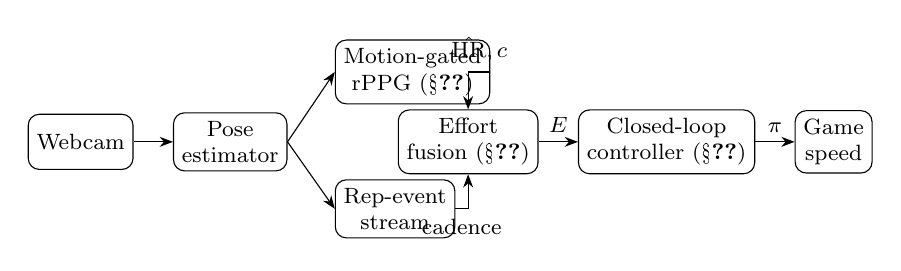
\begin{tikzpicture}[
  font=\footnotesize,
  block/.style={draw,rounded corners,minimum height=7mm,align=center,inner sep=3pt},
  >={Stealth[]}, node distance=4.2mm and 5mm]
\node[block] (cam) {Webcam};
\node[block,right=of cam] (pose) {Pose\\estimator};
\node[block,above right=1mm and 6mm of pose] (rppg) {Motion-gated\\rPPG (\S\ref{sec:rppg})};
\node[block,below right=1mm and 6mm of pose] (rep) {Rep-event\\stream};
\node[block,right=14mm of pose] (effort) {Effort\\fusion (\S\ref{sec:effort})};
\node[block,right=of effort] (ctrl) {Closed-loop\\controller (\S\ref{sec:control})};
\node[block,right=of ctrl] (game) {Game\\speed};
\draw[->] (cam) -- (pose);
\draw[->] (pose.east) -- (rppg.west);
\draw[->] (pose.east) -- (rep.west);
\draw[->] (rppg.east) -| node[above,pos=0.25]{$\hat{\mathrm{HR}},c$} (effort.north);
\draw[->] (rep.east)  -| node[below,pos=0.25]{cadence} (effort.south);
\draw[->] (effort) -- node[above]{$E$} (ctrl);
\draw[->] (ctrl) -- node[above]{$\pi$} (game);
\end{tikzpicture}
\caption{Wearable-free signal flow. A single pose feed is reused for both motion
control (game speed) and physiological sensing; the skeleton's velocity gates the
rPPG estimate. Architecture details are in~\cite{fitarcade-sdps}.}
\label{fig:signalflow}
\end{figure}

% =====================================================================
\section{Motion-Gated rPPG Method}\label{sec:rppg}
The estimator maintains a rolling window of $W=10$\,s of per-frame ROI colour
means, recomputing HR at most once per second once at least $N_{\min}=60$ samples
are buffered. Fig.~\ref{fig:rppgblock} summarizes the pipeline;
Algorithm~\ref{alg:rppg} gives the procedure.

\subsection{Pose-Reuse Forehead ROI}
Rather than run a separate face detector, the ROI is derived from the pose face
landmarks: nose $\mathbf{p}_0$, eyes $\mathbf{p}_2,\mathbf{p}_5$, and ears
$\mathbf{p}_7,\mathbf{p}_8$ (normalized image coordinates). With eye line
$y_e=(p_{2,y}+p_{5,y})/2$ and a face-width proxy
$w_f=\max(|p_{7,x}-p_{8,x}|,\,0.06)$, a forehead box of size
$(0.55w_f)\times(0.45w_f)$ is centred horizontally at the nose and vertically at
$y_e-0.35w_f$, clamped to the frame. The box is resampled to a $48\times48$ patch
and averaged to per-frame channel means $(R_i,G_i,B_i)$ at timestamp $t_i$.

\subsection{Extractor-Agnostic Pulse Signal}
Over the current window of $N$ samples, let $\bar C=\tfrac1N\sum_i C_i$ for
$C\in\{R,G,B\}$ and mean-normalize $C_n[i]=C_i/\bar C-1$. A pluggable
\emph{extractor} maps the normalized channels to a scalar pulse $h[i]$. Because
the motion-gating contribution below is independent of this choice, the front-end
can be selected to trade accuracy, complexity, and licensing: the deployed system
defaults to green-channel plethysmography~\cite{verkruysse2008},
$h_{\text{green}}[i]=G_n[i]$, and we additionally support two chrominance
projections as evaluation baselines (Study~3). CHROM~\cite{dehaan2013} forms
\begin{align}
X[i] &= 3R_n[i]-2G_n[i], & Y[i] &= 1.5R_n[i]+G_n[i]-1.5B_n[i],
\end{align}
with $h_{\text{chrom}}=X-\alpha Y$ and $\alpha=\sigma(X)/\sigma(Y)$; POS~\cite{wang2017} forms
\begin{align}
S_1[i] &= G_n[i]-B_n[i], & S_2[i] &= -2R_n[i]+G_n[i]+B_n[i],
\end{align}
with $h_{\text{pos}}=S_1+\alpha S_2$ and $\alpha=\sigma(S_1)/\sigma(S_2)$ (ratios of
standard deviations over the window). In all cases the pulse is detrended and
Hann-windowed,
\begin{equation}
\tilde h[i] = \bigl(h[i]-\bar h\bigr)\Bigl[0.5-0.5\cos\tfrac{2\pi i}{N-1}\Bigr].
\end{equation}

\subsection{Non-Uniform Periodogram and Confidence}
Webcam frame timing is irregular, so we avoid a uniform-grid FFT and evaluate a
direct periodogram on the true relative timestamps $\tau_i=t_i-t_0$ over integer
beats-per-minute $b$:
\begin{equation}
P(b)=\!\Bigl(\sum_i \tilde h[i]\cos 2\pi\tfrac{b}{60}\tau_i\Bigr)^2
      +\Bigl(\sum_i \tilde h[i]\sin 2\pi\tfrac{b}{60}\tau_i\Bigr)^2,
\end{equation}
for $b\in\{40,\dots,180\}$\,bpm. The peak gives the instantaneous estimate
$\hat b=\arg\max_b P(b)$, and a spectral peak-to-mean ratio gives a raw confidence
\begin{equation}
c_0=\min\!\Bigl(1,\ \frac{P(\hat b)}{8\,\bar P}\Bigr),\qquad
\bar P=\frac{1}{|B|}\sum_{b\in B}P(b).
\label{eq:conf}
\end{equation}

\subsection{Pose-Velocity Motion Gate (novel)}
The nose landmark speed between frames,
$s=\lVert\mathbf{p}_0[t]-\mathbf{p}_0[t-1]\rVert/\Delta t$ (normalized units per
second), is exponentially smoothed into a motion level
\begin{equation}
m \leftarrow 0.7\,m + 0.3\,s .
\end{equation}
A motion penalty linearly attenuates confidence above threshold $\tau=0.12$ and
zeros it once motion dominates,
\begin{equation}
\rho=\max\!\Bigl(0,\ 1-\frac{m}{\tau}\Bigr),\qquad c=c_0\,\rho .
\label{eq:gate}
\end{equation}
The estimate is updated only when trusted, and \emph{held} otherwise:
\begin{equation}
\hat{\mathrm{HR}}\leftarrow
\begin{cases}
0.7\,\hat{\mathrm{HR}}+0.3\,\hat b, & c\ge 0.25\ \text{(and }\hat{\mathrm{HR}}{>}0),\\
\hat b, & c\ge 0.25\ \text{(first estimate)},\\
\hat{\mathrm{HR}}, & c<0.25\ \text{(hold)}.
\end{cases}
\label{eq:hold}
\end{equation}
Personalization sets $\hmax=220-a$ for age $a$; the training zone is
$\mathrm{zone}(\hat{\mathrm{HR}})$ from $\hat{\mathrm{HR}}/\hmax$ with thresholds
$\{0.5,0.6,0.7,0.85\}$ (REST/WARM/FAT-BURN/CARDIO/PEAK).

\begin{figure}[t]
\centering
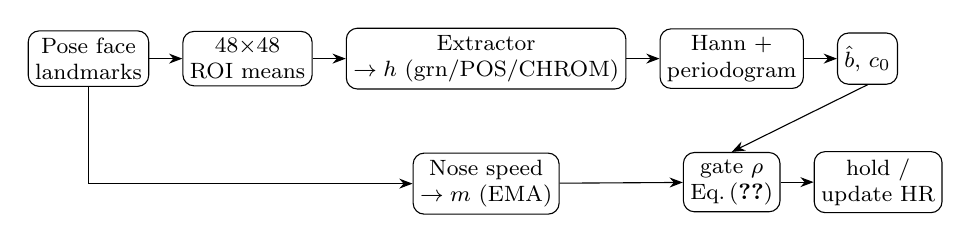
\begin{tikzpicture}[font=\footnotesize,
  b/.style={draw,rounded corners,align=center,minimum height=6.5mm,inner sep=2.5pt},
  >={Stealth[]}, node distance=3.4mm and 4.2mm]
\node[b] (roi) {Pose face\\landmarks};
\node[b,right=of roi] (rgb) {$48{\times}48$\\ROI means};
\node[b,right=of rgb] (pos) {Extractor\\$\to h$ (grn/POS/CHROM)};
\node[b,right=of pos] (per) {Hann +\\periodogram};
\node[b,right=of per] (hr)  {$\hat b,\,c_0$};
\node[b,below=8mm of pos] (mot) {Nose speed\\$\to m$ (EMA)};
\node[b,below=8mm of per] (gate){gate $\rho$\\Eq.\,\eqref{eq:gate}};
\node[b,right=of gate] (out) {hold /\\update HR};
\draw[->](roi)--(rgb);\draw[->](rgb)--(pos);\draw[->](pos)--(per);\draw[->](per)--(hr);
\draw[->](roi.south)|-(mot.west);
\draw[->](mot)--(gate);\draw[->](hr.south)--(gate.north);
\draw[->](gate)--(out);
\end{tikzpicture}
\caption{Motion-gated rPPG. The pose skeleton supplies both the ROI (top path) and
the motion observable (bottom path) that gates confidence and holds the estimate.}
\label{fig:rppgblock}
\end{figure}

\begin{algorithm}[t]
\caption{Motion-gated rPPG (per compute tick)}\label{alg:rppg}
\begin{algorithmic}[1]
\Require ring buffer $\{(t_i,R_i,G_i,B_i)\}_{i=1}^{N}$, motion level $m$
\State drop samples older than $W{=}10$\,s; \textbf{if} $N<N_{\min}{=}60$ \textbf{return}
\State $C_n[i]\gets C_i/\bar C-1$ for $C\in\{R,G,B\}$
\State $h\gets \textsc{Extract}(R_n,G_n,B_n)$ \Comment{green (default) / CHROM / POS}
\State detrend; Hann window $\to\tilde h$
\State $P(b)\gets$ periodogram on timestamps $\tau_i$, $b\in[40,180]$
\State $\hat b\gets\arg\max P$;\ \ $c_0\gets\min(1,P(\hat b)/8\bar P)$ \Comment{Eq.\,\eqref{eq:conf}}
\State $\rho\gets\max(0,1-m/\tau)$;\ \ $c\gets c_0\rho$ \Comment{Eq.\,\eqref{eq:gate}}
\If{$c\ge 0.25$} update $\hat{\mathrm{HR}}$ (EMA $0.7/0.3$); recompute zone
\Else{} \textbf{hold} $\hat{\mathrm{HR}}$ \Comment{Eq.\,\eqref{eq:hold}}
\EndIf
\State \Return $\hat{\mathrm{HR}},\,c,\,\mathrm{zone}$
\end{algorithmic}
\end{algorithm}

% =====================================================================
\section{Effort Estimation}\label{sec:effort}
Effort $E\in[0,1]$ is updated each second by fusing two markerless sources.
\emph{Cadence:} rep events over a $W_e=20$\,s window give
$\mathrm{rpm}=r\cdot 60/W_e$ for $r$ reps, normalized against an ``all-out''
$r_{\max}=50$\,rpm,
\begin{equation}
u_{\text{cad}}=\clip\!\bigl(\mathrm{rpm}/r_{\max},\,0,\,1\bigr).
\end{equation}
\emph{HR reserve:} when HR is trustworthy ($\hat{\mathrm{HR}}>0$ and $c\ge0.3$),
\begin{equation}
u_{\text{hr}}=\clip\!\Bigl(\frac{\hat{\mathrm{HR}}-\hrrest}{\hmax-\hrrest},\,0,\,1\Bigr).
\end{equation}
The instantaneous effort blends the two, falling back to cadence alone when HR is
untrusted:
\begin{equation}
u=\begin{cases}
0.5\,u_{\text{cad}}+0.5\,u_{\text{hr}}, & \hat{\mathrm{HR}}>0 \wedge c\ge 0.3,\\[2pt]
u_{\text{cad}}, & \text{otherwise},
\end{cases}
\end{equation}
and is exponentially smoothed to avoid twitchy adaptation:
\begin{equation}
E\leftarrow 0.6\,E + 0.4\,u.
\end{equation}
The confidence gate here ($0.3$) is stricter than the rPPG hold gate ($0.25$):
HR is displayed once minimally trusted but only \emph{fused into effort} when more
strongly trusted, so noisy HR never inflates the control signal.

% =====================================================================
\section{Personalized Closed-Loop Adaptation}\label{sec:control}
\subsection{Control Law}
A discrete integral-type controller nudges a difficulty multiplier $d$ toward a
per-phase effort target $\theta_\phi$ every $T_c=2$\,s:
\begin{equation}
d\leftarrow \clip\!\bigl(d+g\,(\theta_\phi-E),\ d_{\min},\ d_{\max}\bigr),
\quad g=0.18,
\label{eq:control}
\end{equation}
with $d\in[d_{\min},d_{\max}]=[0.85,1.2]$. The command issued to the game is the
personalized baseline scaled by this multiplier,
\begin{equation}
\pi = p_0\cdot d,
\end{equation}
so the game speed can drift only $-15\%$ to $+20\%$ around each player's baseline.
The gain $g$ is deliberately small: unlike a mouse, a real jump, squat, or
push-up cannot be ``spammed,'' so effort responds on the time scale of seconds;
an aggressive gain would oscillate against this slow, rate-limited plant. With
$|\theta_\phi-E|\le1$ and $g=0.18$, a single update moves $d$ by at most $0.18$,
and the clamp bounds the excursion, giving a stable, gently critically-damped
response. \todoNote{optionally add a discrete-time stability note / step-response
figure once logged traces exist.}

\subsection{Per-Phase Targets}
A structured session sequences three phases, each specifying a target effort
band~\cite{fitarcade-sdps}: warm-up $\theta=0.40$, high-intensity $\theta=0.60$,
and cool-down $\theta=0.35$ (a default of $\theta=0.55$ applies to unstructured
play). The controller therefore regulates the player toward a phase-appropriate
relative intensity rather than a fixed speed.

\subsection{Baseline Personalization}
The baseline $p_0$ is computed once per player from age $a$, resting HR
$\hrrest$, and self-reported fitness level:
\begin{align}
f_{\text{age}} &= \clip\!\bigl(1-0.3\,\tfrac{\max(0,a-20)}{50},\,0.7,\,1.0\bigr),\\
f_{\text{fit}} &= \begin{cases}0.85 & \text{beginner}\\ 1.00 & \text{intermediate}\\ 1.15 & \text{advanced}\end{cases}\\
f_{\text{rhr}} &= \clip\!\bigl(1+\tfrac{60-\hrrest}{400},\,0.94,\,1.06\bigr),\\
p_0 &= \clip\!\bigl(f_{\text{age}}\,f_{\text{fit}}\,f_{\text{rhr}},\,0.55,\,1.2\bigr).
\end{align}
The same age sets $\hmax=220-a$, coupling the personalization of pace to the
personalization of the HR-reserve scale. Table~\ref{tab:personalization} shows
worked baselines spanning the profile space; a fit 22-year-old starts $\sim$2$\times$
faster than a deconditioned 65-year-old, and the closed loop then adapts around
each anchor. Algorithm~\ref{alg:effctrl} summarizes effort fusion and control.

\begin{table}[t]
\caption{Personalized baseline pace $p_0$ (from \texttt{computeBasePace}) and
$\hmax$ across representative profiles.}
\label{tab:personalization}
\centering
\footnotesize
\begin{tabular}{@{}lccccc@{}}
\toprule
Profile (age / rest / fitness) & $f_{\text{age}}$ & $f_{\text{fit}}$ & $f_{\text{rhr}}$ & $p_0$ & $\hmax$\\
\midrule
22 / 50 / advanced      & 0.99 & 1.15 & 1.025 & 1.16 & 198\\
25 / 60 / beginner      & 0.97 & 0.85 & 1.000 & 0.82 & 195\\
35 / 65 / intermediate  & 0.91 & 1.00 & 0.988 & 0.90 & 185\\
50 / 70 / beginner      & 0.82 & 0.85 & 0.975 & 0.68 & 170\\
65 / 75 / beginner      & 0.73 & 0.85 & 0.963 & 0.60 & 155\\
\bottomrule
\end{tabular}
\end{table}

\begin{algorithm}[t]
\caption{Effort fusion + closed-loop difficulty (per $T_c$)}\label{alg:effctrl}
\begin{algorithmic}[1]
\Require rep times, $\hat{\mathrm{HR}},c$, phase target $\theta_\phi$, baseline $p_0$
\State $\mathrm{rpm}\gets 60\,r/W_e$;\ \ $u_{\text{cad}}\gets\clip(\mathrm{rpm}/50,0,1)$
\If{$\hat{\mathrm{HR}}>0 \wedge c\ge0.3$}
  \State $u_{\text{hr}}\gets\clip((\hat{\mathrm{HR}}-\hrrest)/(\hmax-\hrrest),0,1)$
  \State $u\gets 0.5u_{\text{cad}}+0.5u_{\text{hr}}$
\Else{}\ $u\gets u_{\text{cad}}$
\EndIf
\State $E\gets 0.6E+0.4u$
\State $d\gets\clip(d+0.18(\theta_\phi-E),0.85,1.2)$ \Comment{Eq.\,\eqref{eq:control}}
\State emit command $\pi\gets p_0\,d$ to game
\end{algorithmic}
\end{algorithm}

% =====================================================================
\section{Experimental Design}\label{sec:design}
We describe a pre-registered\footnote{\todoNote{register protocol/hypotheses
before data collection.}} human-subjects protocol. Because no data are yet
collected, quantitative cells below are placeholders (\result{blue}); none are
fabricated.

\subsection{Participants and Ethics}
$N=\ph{N=32}$ healthy adults (power justification: \todoNote{report target effect
size, $\alpha$, power, and the analysis the calculation targets}) recruited to span
the Fitzpatrick skin-tone scale I--VI and a range of age/fitness. Ethics approval:
\ph{IRB\_NUMBER}; written informed consent and PAR-Q screening precede
participation.

\subsection{Apparatus and Ground Truth}
Reference HR: \ph{REFERENCE\_DEVICE, e.g.\ Polar~H10 ECG chest strap}, time-
synchronized to the video stream (\todoNote{state sync method and residual offset}).
Camera: \ph{CAMERA\_SPEC} at \ph{FPS}\,fps, participant at \ph{D}\,m, under
\ph{lighting conditions}. All rPPG variants are computed offline from the same
recordings for a fair comparison. Perceived exertion via Borg RPE~\cite{borg1982};
player experience via the Intrinsic Motivation Inventory~\cite{imi} and a
flow/GameFlow instrument~\cite{gameflow}.

\subsection{Studies, Metrics, Statistics}
\begin{itemize}
\item \textbf{S1 --- HR accuracy.} Rest and each game; MAE, RMSE, Bland--Altman
limits of agreement, Pearson $r$; stratified by skin tone, lighting, and motion
intensity.
\item \textbf{S2 --- Motion-gating ablation (headline).} Gated
(Eqs.~\eqref{eq:gate}--\eqref{eq:hold}) vs.\ ungated during vigorous play: error
reduction and the coverage-vs.\ hold-time trade-off (fraction of time held, error
during held vs.\ live spans).
\item \textbf{S3 --- rPPG baselines.} Green~\cite{verkruysse2008},
CHROM~\cite{dehaan2013}, ICA~\cite{poh2010}, POS~\cite{wang2017}, and a
deep-learning baseline (DeepPhys~\cite{chen2018}/PhysNet~\cite{yu2019}) under
identical inputs; subject-independent (leave-one-subject-out) evaluation.
\item \textbf{S4 --- Effort validity.} Fused $E$ vs.\ \%HRR and Borg RPE;
correlation and agreement.
\item \textbf{S5 --- Closed-loop efficacy.} Adaptive vs.\ fixed difficulty
(within-subjects, counterbalanced): time-in-target-HR-zone, flow, enjoyment (IMI),
and moderate-to-vigorous minutes.
\item \textbf{S6 --- Personalization.} Whether $p_0$ yields comparable
\emph{relative} intensity (\%HRR) across age/fitness groups.
\end{itemize}
Analyses use linear mixed-effects models with participant random effects;
we report effect sizes with 95\% confidence intervals and correct for multiple
comparisons (\todoNote{state method, e.g.\ Holm--Bonferroni}).

% =====================================================================
\section{Results}\label{sec:results}
\emph{All quantitative results are placeholders pending data collection.}

\textbf{S1 (accuracy).} Overall MAE \result{-- bpm}, RMSE \result{-- bpm},
$r=\result{--}$; Bland--Altman bias \result{--} with LoA
[\result{--},\result{--}]; by skin tone I--III vs.\ IV--VI:
\result{-- vs.\ -- bpm}; Fig.~\ref{fig:bland} (\todoNote{real plot}).

\textbf{S2 (gating ablation).} Gating reduced MAE during vigorous play from
\result{-- bpm} (ungated) to \result{-- bpm} (gated), a \result{--\%} reduction,
holding \result{--\%} of the time; Fig.~\ref{fig:ablation} (\todoNote{real bar
chart}).

\textbf{S3 (baselines).} Table~\ref{tab:baselines}: our gated green-channel
pipeline vs.\ ungated extractors under identical inputs.

\textbf{S4--S6.} Effort--\%HRR $r=\result{--}$, effort--RPE $\rho=\result{--}$;
adaptive increased time-in-zone from \result{--\%} to \result{--\%}
($d=\result{--}$) and \todoNote{report flow/IMI}; relative intensity across
profiles differed by \result{-- \%HRR} (n.s./sig., \todoNote{fill}).

\begin{figure}[t]\centering
\framebox[0.9\linewidth][c]{\rule{0pt}{28mm}\ \ \parbox{0.7\linewidth}{\centering
\textcolor{blue}{Bland--Altman + scatter}\\ \todoNote{insert once data collected}}}
\caption{Agreement between motion-gated rPPG and reference HR.}\label{fig:bland}
\end{figure}

\begin{figure}[t]\centering
\framebox[0.9\linewidth][c]{\rule{0pt}{24mm}\ \ \parbox{0.7\linewidth}{\centering
\textcolor{blue}{Ablation: MAE gated vs.\ ungated by motion band}\\ \todoNote{insert}}}
\caption{Motion-gating ablation (headline).}\label{fig:ablation}
\end{figure}

\begin{table}[t]
\caption{Subject-independent HR accuracy by method (identical inputs).}
\label{tab:baselines}
\centering\footnotesize
\begin{tabular}{@{}lccc@{}}
\toprule
Method & MAE (bpm) & RMSE (bpm) & $r$\\
\midrule
Green~\cite{verkruysse2008}       & \result{--} & \result{--} & \result{--}\\
ICA~\cite{poh2010}                & \result{--} & \result{--} & \result{--}\\
CHROM~\cite{dehaan2013}           & \result{--} & \result{--} & \result{--}\\
POS~\cite{wang2017}               & \result{--} & \result{--} & \result{--}\\
DL~\cite{chen2018}                & \result{--} & \result{--} & \result{--}\\
\textbf{Green + motion gate (ours)} & \result{--} & \result{--} & \result{--}\\
\bottomrule
\end{tabular}
\end{table}

% =====================================================================
\section{Discussion}\label{sec:discussion}
\textbf{What the ablation shows.} If S2 confirms that pose-velocity gating cuts
error during the motion bursts that defeat naive rPPG---at the cost of holding the
estimate for a bounded fraction of time---then a cheap, already-computed observable
substantially closes the gap between rest-grade and exercise-grade contactless HR.
The hold policy trades temporal coverage for reliability; because the downstream
controller updates only every $T_c=2$\,s and effort is heavily smoothed, brief
holds are tolerable.

\textbf{Fairness.} rPPG is known to degrade on darker skin and in poor lighting.
We therefore treat skin tone (Fitzpatrick I--VI) and lighting as first-class
stratification factors in S1/S3, and report per-stratum accuracy rather than
aggregate numbers alone. The deployed green-channel front-end is the simplest and
least encumbered but also the most sensitive to skin tone; Study~3 quantifies the
accuracy cost of the extractor choice, and CHROM/POS remain selectable where their
added robustness justifies the complexity. \todoNote{discuss any observed
disparity and mitigation.}

\textbf{Failure modes and limits.} (i) Sustained maximal motion drives $\rho\to0$
and the estimate is held indefinitely; the effort estimator's cadence fallback
covers this regime but loses cardiovascular information. (ii) The face must remain
visible; occlusion or out-of-frame excursions suspend sensing. (iii) The control
law is intentionally simple; richer plants (e.g., per-game difficulty surfaces)
are future work. (iv) Findings will be lab-based; free-living robustness is
unaddressed. A Threats-to-Validity summary: \todoNote{internal (device sync,
author-run sessions), external (in-house games, single site), construct (effort
proxy), and statistical (multiplicity, sample size) threats.}

% =====================================================================
\section{Conclusion}\label{sec:conclusion}
We presented a wearable-free sensing-and-adaptation pipeline for markerless
exergaming in which the body pose the game already computes is reused to make
contactless HR robust to the vigorous motion that normally defeats it, to fuse a
markerless effort signal, and to drive a personalized closed-loop difficulty
controller. The method is fully specified and grounded in a deployed
implementation; a rigorous, pre-registered evaluation with accuracy, ablation,
baseline, validity, efficacy, and personalization studies is defined, with
quantitative outcomes to follow data collection. Future work includes deep-model
gating, free-living validation, and richer control.

% =====================================================================
\section*{Acknowledgment}
\todoNote{funding, participants, ethics board.}

\bibliographystyle{IEEEtran}
\bibliography{refs}

\end{document}
